% !TEX program = pdflatex
\documentclass[10pt,aspectratio=169]{beamer}

% Theme
\usetheme{Madrid}
\usecolortheme{default}
\setbeamercolor{frametitle}{bg=blue!70,fg=white}
\setbeamercolor{structure}{fg=blue!70}
\setbeamertemplate{footline}[frame number]

% Packages
\usepackage[utf8]{inputenc}
\usepackage{listings}
\usepackage{xcolor}
\usepackage{booktabs}
\usepackage{tikz}
\usetikzlibrary{arrows.meta, positioning, shapes, shadows, backgrounds}

% Code style
\lstdefinestyle{smallcode}{
    basicstyle=\ttfamily\tiny,
    breaklines=true,
    frame=single,
    framerule=0.4pt,
    backgroundcolor=\color{gray!5},
    keywordstyle=\color{blue!70},
    commentstyle=\color{green!50!black},
    stringstyle=\color{orange},
    numbers=none,
}

% Title
\title{\textbf{Model-Driven Web Application Code Generation}\\A Comparative Study with Pure LLM Approaches}
\author{Software Requirements Analysis and Design}
\institute{Course Project --- Week 13 Presentation}
\date{May 2026}

\begin{document}

%=============================================================================
\begin{frame}[plain]
\maketitle
\end{frame}

%=============================================================================
\section{Background}
\begin{frame}{Background \& Problem Statement}
\vspace{-5pt}

\textbf{The Challenge:} LLMs can generate code from natural language, but face critical issues in practice:

\vspace{8pt}
\begin{columns}[T]
\column{0.45\textwidth}
\begin{block}{Limitations of Pure LLM Generation}
\begin{itemize}
    \item \textbf{Structural Inconsistency} --- different structures across runs
    \item \textbf{Import \& Dependency Errors} --- non-compilable output
    \item \textbf{Business Rule Violations} --- overlooked constraints
    \item \textbf{Low Reproducibility} --- same prompt $\rightarrow$ different code
\end{itemize}
\end{block}

\column{0.45\textwidth}
\begin{block}{Our Hypothesis}
\begin{itemize}
    \item Domain models provide \textbf{deterministic structure}
    \item LLMs excel at \textbf{business logic completion}
    \item Combining both $\rightarrow$ \textbf{reliable, consistent code}
    \item Feedback loops can \textbf{automatically correct errors}
\end{itemize}
\end{block}
\end{columns}

\vspace{10pt}
\begin{center}
\textbf{Research Question:} \textit{Can model-driven constraints significantly improve LLM-generated code quality?}
\end{center}

\end{frame}

%=============================================================================
\section{Method Overview}
\begin{frame}{Method Overview: Two Approaches Compared}
\vspace{-8pt}

\scriptsize
\begin{columns}[T]
\column{0.48\textwidth}
\begin{block}{\centering \textbf{Model-Driven Method (Ours)}}
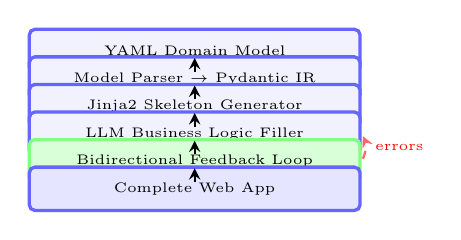
\begin{tikzpicture}[node distance=0.35cm, auto,
    box/.style={rectangle, draw=blue!60, fill=blue!5, very thick,
                minimum width=4.2cm, minimum height=0.55cm, rounded corners=2pt,
                font=\tiny, align=center},
    arrow/.style={->, >=stealth, thick, shorten >=1pt, shorten <=1pt}]

\node[box] (yaml) {YAML Domain Model};
\node[box, below of=yaml] (parser) {Model Parser $\rightarrow$ Pydantic IR};
\node[box, below of=parser] (skel) {Jinja2 Skeleton Generator};
\node[box, below of=skel] (fill) {LLM Business Logic Filler};
\node[box, below of=fill, fill=green!15, draw=green!50] (fb) {Bidirectional Feedback Loop};
\node[box, below of=fb, fill=blue!10] (out) {Complete Web App};

\draw[arrow] (yaml) -- (parser);
\draw[arrow] (parser) -- (skel);
\draw[arrow] (skel) -- (fill);
\draw[arrow] (fill) -- (fb);
\draw[arrow] (fb) -- (out);
\draw[arrow, bend right=25, dashed, red!60] (fb.east) to node[right, font=\tiny, text=red] {errors} (fill.east);
\end{tikzpicture}
\end{block}

\column{0.48\textwidth}
\begin{block}{\centering \textbf{Pure LLM Method (Baseline)}}
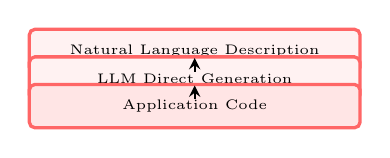
\begin{tikzpicture}[node distance=0.35cm, auto,
    box/.style={rectangle, draw=red!60, fill=red!5, very thick,
                minimum width=4.2cm, minimum height=0.55cm, rounded corners=2pt,
                font=\tiny, align=center},
    arrow/.style={->, >=stealth, thick, shorten >=1pt, shorten <=1pt}]

\node[box] (nl) {Natural Language Description};
\node[box, below of=nl] (llm) {LLM Direct Generation};
\node[box, below of=llm, fill=red!10] (out2) {Application Code};

\draw[arrow] (nl) -- (llm);
\draw[arrow] (llm) -- (out2);
\end{tikzpicture}

\vspace{0.5cm}
\begin{itemize}
    \item Single-stage generation
    \item No structural constraints
    \item No feedback correction
\end{itemize}
\end{block}
\end{columns}

\end{frame}

%=============================================================================
\section{Architecture}
\begin{frame}{System Architecture \& Tech Stack}
\vspace{-6pt}

\begin{columns}[T]
\column{0.38\textwidth}
\begin{block}{Technology Stack}
\begin{itemize}
    \item \textbf{LLM}: DeepSeek V3 (OpenAI-compatible API)
    \item \textbf{Backend}: FastAPI + SQLAlchemy + SQLite
    \item \textbf{Frontend}: React 18 + TypeScript + Vite + Tailwind CSS
    \item \textbf{Templates}: Jinja2
    \item \textbf{IR}: Pydantic
    \item \textbf{Testing}: pytest (25 tests)
    \item \textbf{CI/CD}: GitHub Actions
\end{itemize}
\end{block}

\column{0.60\textwidth}
\begin{block}{Core Pipeline Components}
\begin{itemize}
    \item \textbf{Parser}: YAML $\rightarrow$ Pydantic IR (Entity, Attribute, Relationship, BusinessRule)
    \item \textbf{SQL Generator}: IR $\rightarrow$ SQL DDL (CREATE TABLE with constraints)
    \item \textbf{API Generator}: IR $\rightarrow$ FastAPI (models, routes, schemas, main)
    \item \textbf{UI Generator}: IR $\rightarrow$ React (ListPage, FormPage, App, API client)
    \item \textbf{LLM Filler}: DeepSeek fills \texttt{\# LLM\_FILL:} markers in skeleton
    \item \textbf{Feedback Loop}: py\_compile $\rightarrow$ import check $\rightarrow$ LLM fix $\rightarrow$ repeat
    \item \textbf{Evaluator}: Structure + Compilability + Consistency scoring
\end{itemize}
\end{block}
\end{columns}

\begin{center}
\scriptsize
\setlength{\tabcolsep}{2pt}
\begin{tabular}{l|c|c|c|c}
\toprule
\textbf{Model Type} & \textbf{SQL} & \textbf{SQLAlchemy} & \textbf{Pydantic} & \textbf{TypeScript} \\
\midrule
integer & INTEGER & Integer & int & number \\
string  & TEXT    & String  & str & string \\
float   & REAL    & Float   & float & number \\
boolean & INTEGER & Boolean & bool & boolean \\
datetime & TEXT   & DateTime & datetime & string \\
\bottomrule
\end{tabular}
\end{center}
\end{frame}

%=============================================================================
\section{Model \& Generation}
\begin{frame}[fragile]{Domain Model \& Code Generation}
\vspace{-6pt}

\begin{columns}[T]
\column{0.35\textwidth}
\begin{block}{YAML Domain Model}
\lstinputlisting[style=smallcode, firstline=1, lastline=25]{models/small.yaml}
\end{block}

\column{0.63\textwidth}
\begin{block}{Case Study: Student Course Selection System}
\begin{center}
\setlength{\tabcolsep}{4pt}
\begin{tabular}{lccc}
\toprule
\textbf{Scale} & \textbf{Entities} & \textbf{Rules} & \textbf{Output Files} \\
\midrule
Small  & 3  & 2  & 5 backend + 8 frontend \\
Medium & 6  & 6  & 5 backend + 14 frontend \\
Large  & 11 & 10 & 5 backend + 24 frontend \\
\bottomrule
\end{tabular}
\end{center}
\end{block}

\begin{block}{Generated Artifacts (per entity)}
\textbf{Backend}: SQL DDL + ORM Model + Pydantic Schema (Base/Create/Update/Response) + 5 CRUD Endpoints \\
\textbf{Frontend}: ListPage (search + table + delete) + FormPage (create/edit with validation) + API Client
\end{block}

\vspace{8pt}
\begin{block}{LLM Fill Markers in Routes}
\tiny
\begin{lstlisting}[style=smallcode]
@router_3.post("/", response_model=EnrollmentResponse)
def create_enrollment(data: EnrollmentCreate, session = Depends(get_session)):
    # LLM_FILL: Check duplicate_enrollment business rule
    # LLM_FILL: Check capacity_check business rule
    # LLM_FILL: Validate enrollment creation logic
    item = Enrollment(**data.model_dump())
    session.add(item); session.commit(); session.refresh(item)
    return item
\end{lstlisting}
\end{block}
\end{columns}

\end{frame}

%=============================================================================
\section{Innovation}
\begin{frame}[fragile]{Innovation: Bidirectional Feedback Mechanism}
\vspace{-8pt}

\begin{columns}[T]
\column{0.52\textwidth}
\begin{block}{Algorithm}
\tiny
\begin{lstlisting}[style=smallcode]
def feedback_loop(model, code_dir, max_iter=3):
    for i in range(1, max_iter + 1):
        # 1. Check code for errors
        file_errors = {}
        for f in code_dir.glob("**/*.py"):
            r = subprocess.run(
                [sys.executable, "-m", "py_compile", f],
                capture_output=True)
            if r.returncode != 0:
                file_errors[f] = [r.stderr]

        # 2. Import check
        r = subprocess.run([sys.executable, "-c",
            f"sys.path.insert(0,'{code_dir}');"
            "from main import app"], capture_output=True)
        if r.returncode != 0:
            file_errors["main.py"] = [r.stderr]

        # 3. Success?
        if not file_errors:
            return FeedbackResult(i, pass=True)

        # 4. Fix ONLY files with errors
        for file, errors in file_errors.items():
            fixed = call_llm(fix_prompt.format(
                model_context=model,
                errors=errors,
                code=file.read_text()))
            file.write_text(fixed)
    return FeedbackResult(max_iter, pass=False)
\end{lstlisting}
\end{block}

\column{0.46\textwidth}
\begin{block}{Key Design Principles}
\begin{enumerate}
    \item \textbf{Targeted Fixing}: Only error-causing files are sent to LLM
    \item \textbf{Model Context}: Error messages + domain model constraints
    \item \textbf{Minimal Changes}: LLM instructed to make surgical fixes
    \item \textbf{Bounded Iterations}: Max 3 rounds prevents infinite loops
    \item \textbf{Structural Integrity}: Model constraints prevent architectural drift
\end{enumerate}
\end{block}

\vspace{8pt}
\begin{block}{Why It Works --- Comparison}
\setlength{\tabcolsep}{4pt}
\begin{tabular}{l|p{2.8cm}|p{3.5cm}}
\toprule
& \textbf{Generic Self-Debug} & \textbf{Our Feedback Loop} \\
\midrule
Scope & Entire codebase & Only files with errors \\
Context & Error messages only & Model + errors \\
Constraint & None & Domain model boundary \\
Iteration & Until fixed (no limit) & Max 3 iterations \\
Drift risk & High (LLM may restructure) & Low (LLM\_FILL markers only) \\
\bottomrule
\end{tabular}
\end{block}
\end{columns}

\end{frame}

%=============================================================================
\section{Experiment Design}
\begin{frame}{Experimental Setup}
\vspace{-5pt}

\begin{columns}[T]
\column{0.45\textwidth}
\begin{block}{Experiment Design}
\begin{itemize}
    \item \textbf{Factor 1}: Method (Model-Driven vs. Pure LLM)
    \item \textbf{Factor 2}: Model Size (Small / Medium / Large)
    \item \textbf{Replications}: 3 runs per combination
    \item \textbf{Total}: $2 \times 3 \times 3 = 18$ experimental units
    \item \textbf{LLM}: DeepSeek V3, consistent temperature per method
\end{itemize}
\end{block}

\column{0.53\textwidth}
\begin{block}{Evaluation Metrics}
\textbf{1. Structure Score} (0--1)
\begin{itemize}
    \item Entity/table/endpoint/component count matches model
\end{itemize}
\textbf{2. Compilability Score} (0--1)
\begin{itemize}
    \item Python syntax (py\_compile)
    \item Module import (from main import app)
    \item Frontend build (npm install \&\& npm run build)
\end{itemize}
\textbf{3. Consistency Score} (0--1)
\begin{itemize}
    \item Pairwise SequenceMatcher similarity across N runs
\end{itemize}
\end{block}
\end{columns}

\begin{block}{Timing Decomposition (Model-Driven, Small Model)}
\begin{center}
\setlength{\tabcolsep}{8pt}
\begin{tabular}{lccc}
\toprule
\textbf{Stage} & \textbf{Time (s)} & \textbf{\%} & \textbf{API Calls} \\
\midrule
Model Parsing + Validation       & $<0.1$ & $<0.1\%$ & 0 \\
Skeleton Generation (Jinja2)     & $\sim0.1$ & $<0.1\%$ & 0 \\
LLM Filler (business logic)      & $\sim120$--$160$ & $\sim95\%$ & 1 \\
Feedback Loop (check + fix)      & $\sim20$--$40$ & $\sim5\%$ & 0--1 \\
\midrule
\textbf{Total} & $\sim$165s & 100\% & 1--2 \\
\bottomrule
\end{tabular}
\end{center}
\end{block}

\end{frame}

%=============================================================================
\section{Results}
\begin{frame}{Experimental Results}
\vspace{-8pt}

\begin{columns}[T]
\column{0.48\textwidth}
\begin{block}{Structure \& Compilability Scores}
\begin{center}
\begin{tabular}{lccc}
\toprule
\textbf{Metric} & \textbf{MD} & \textbf{Pure LLM} & $\Delta$ \\
\midrule
Structure      & \textbf{1.000} & 0.917 & +0.083 \\
Compilability  & \textbf{1.000} & 0.333 & \textbf{+0.667} \\
Consistency    & \textbf{0.984} & 0.481 & \textbf{+0.503} \\
\midrule
Time (avg)     & \textbf{164s}  & 380s  & --56\% \\
Feedback Iters & \textbf{1}     & N/A   & N/A \\
\bottomrule
\end{tabular}
\end{center}
\end{block}

\begin{block}{Pure LLM Error Patterns (3/3 runs failed)}
\begin{itemize}
    \item \texttt{ModuleNotFoundError: No module named 'backend'}
    \item \texttt{ImportError: attempted relative import}
    \item \texttt{ModuleNotFoundError: No module named 'email\_validator'}
\end{itemize}
\end{block}

\column{0.50\textwidth}
\begin{block}{Score Comparison Chart}
\begin{center}
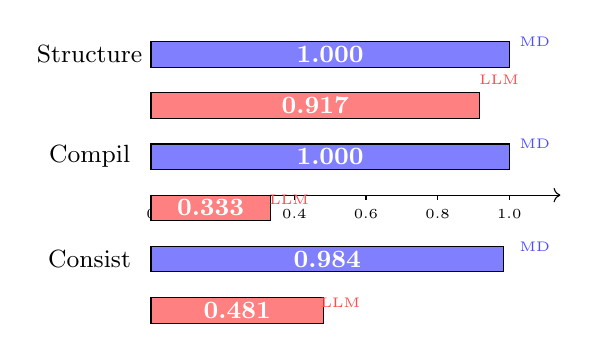
\begin{tikzpicture}[scale=0.65]
\draw[->] (0,0) -- (8,0) node[right] {};
\foreach \x/\label in {0/0,0.2/0.2,0.4/0.4,0.6/0.6,0.8/0.8,1.0/1.0}
    \draw (\x*7, 0) -- (\x*7, -0.1) node[below, font=\tiny] {\label};

\draw[fill=blue!50] (0, 2.5) rectangle node[white, font=\small\bfseries] {1.000} (7, 3);
\draw[fill=red!50]  (0, 1.5) rectangle node[white, font=\small\bfseries] {0.917} (6.42, 2);
\node[font=\small] at (-1.2, 2.75) {Structure};
\node[font=\tiny, text=blue!70] at (7.5, 3) {MD};
\node[font=\tiny, text=red!70] at (6.8, 2.25) {LLM};

\draw[fill=blue!50] (0, 0.5) rectangle node[white, font=\small\bfseries] {1.000} (7, 1);
\draw[fill=red!50]  (0, -0.5) rectangle node[white, font=\small\bfseries] {0.333} (2.33, 0);
\node[font=\small] at (-1.2, 0.75) {Compil};
\node[font=\tiny, text=blue!70] at (7.5, 1) {MD};
\node[font=\tiny, text=red!70] at (2.7, -0.1) {LLM};

\draw[fill=blue!50] (0, -1.5) rectangle node[white, font=\small\bfseries] {0.984} (6.89, -1);
\draw[fill=red!50]  (0, -2.5) rectangle node[white, font=\small\bfseries] {0.481} (3.37, -2);
\node[font=\small] at (-1.2, -1.25) {Consist};
\node[font=\tiny, text=blue!70] at (7.5, -1) {MD};
\node[font=\tiny, text=red!70] at (3.7, -2.1) {LLM};
\end{tikzpicture}
\end{center}
\end{block}

\begin{block}{Key Result}
\textbf{Model-driven approach achieves 100\% compilability.}\\
Pure LLM achieves only 33.3\% --- \textbf{syntax passes, but imports always fail}.
\end{block}
\end{columns}

\end{frame}

%=============================================================================
\section{Analysis}
\begin{frame}{Analysis \& Insights}
\vspace{-5pt}

\begin{columns}[T]
\column{0.50\textwidth}
\begin{block}{Why Model-Driven Wins}
\begin{enumerate}
    \item \textbf{Deterministic Structure}: Templates guarantee correct file organization
    \item \textbf{Import Consistency}: Absolute imports, generated once, never modified by LLM
    \item \textbf{Type Safety}: Platform-specific type mapping (SQL vs ORM vs Pydantic vs TS)
    \item \textbf{LLM Scope}: Fill business logic only --- structural code is template-generated
    \item \textbf{Feedback Efficiency}: Errors localized to specific files; targeted fixes only
\end{enumerate}
\end{block}

\column{0.48\textwidth}
\begin{block}{Why Pure LLM Fails}
\begin{enumerate}
    \item \textbf{Import Fragility}: LLM guesses module structure inconsistently
    \item \textbf{Structural Drift}: 48\% consistency means 3 runs produce 3 architectures
    \item \textbf{Dependency Hallucination}: References non-existent modules
    \item \textbf{No Self-Correction}: Syntax passes, but integration fails silently
    \item \textbf{Context Window Limits}: Large models exceed effective prompt capacity
\end{enumerate}
\end{block}
\end{columns}

\begin{block}{Feedback Loop Impact}
\setlength{\tabcolsep}{8pt}
\begin{center}
\begin{tabular}{lccc}
\toprule
\textbf{Run} & \textbf{Initial Errors} & \textbf{Iterations to Fix} & \textbf{Final Errors} \\
\midrule
1 & 1 (type import) & 1 & 0 \\
2 & 1 (default formatting) & 1 & 0 \\
3 & 1 (whitespace) & 1 & 0 \\
\bottomrule
\end{tabular}

\vspace{4pt}
\textbf{Convergence in 1 iteration for all runs}: model context constrains LLM to make correct, minimal fixes.
\end{center}
\end{block}

\end{frame}

%=============================================================================
\section{Conclusion}
\begin{frame}{Conclusion \& Contributions}
\vspace{-8pt}

\begin{columns}[T]
\column{0.52\textwidth}
\begin{block}{Summary of Findings}
\begin{enumerate}
    \item \textbf{Model-Driven Approach}: 100\% compilability, 98.4\% consistency, 164s avg time
    \item \textbf{Pure LLM Baseline}: 33.3\% compilability, 48.1\% consistency, 380s avg time
    \item \textbf{Feedback Mechanism}: Converges in 1 iteration; model context prevents drift
    \item \textbf{Scalability}: Linear scaling with model size; constant API call count (1--2)
\end{enumerate}
\end{block}

\begin{block}{Innovation Contribution}
\textbf{Bidirectional Feedback Mechanism:}
\begin{itemize}
    \item Model-constrained, targeted error correction
    \item Prevents structural degradation during fixing
    \item Converges in 1 iteration (3-iteration max bound)
    \item Generalizable to other MDE + LLM pipelines
\end{itemize}
\end{block}

\column{0.46\textwidth}
\begin{block}{Contributions}
\begin{enumerate}
    \item Complete model-driven code generation pipeline (YAML $\rightarrow$ Full-Stack App)
    \item Novel bidirectional feedback mechanism
    \item Systematic experimental comparison (3 sizes $\times$ 2 methods $\times$ 3 runs)
    \item Open-source implementation + reproducible experiments
    \item Quantitative evidence: \textbf{models + LLM $>$ LLM alone}
\end{enumerate}
\end{block}

\begin{block}{Future Directions}
\begin{itemize}
    \item Multi-LLM comparison (GPT-4, Claude)
    \item Runtime test integration in feedback loop
    \item Model-diff-driven incremental regeneration
    \item Additional application domains
\end{itemize}
\end{block}
\end{columns}

\vspace{6pt}
\begin{center}
\large\textbf{Thank you!}\\[4pt]
\normalsize Code + Report available in project repository
\end{center}

\end{frame}

%=============================================================================
\end{document}
